\documentclass[journal,harvard,english]{sbatex}
\usepackage{amssymb,amsmath,graphicx,float,array,ae}
\usepackage[latin1]{inputenc}

\newcommand\real{\mathbb{R}}
\newcommand{\req}[1]{(\ref{#1})}
\newcommand{\fimex}{\hfill $\Box$}
\newcounter{examplecounter}
\newtheorem{ex}{Example\refstepcounter{examplecounter}}

\volume{666}
\numero{666}
\mes{April}
\ano{2666}

\begin{document}

\title{Trajectory Tracking of Wheeled Mobile Robots Using Model Predictive Control}

\author{Felipe K�hne}{kuhne@eletro.ufrgs.br}
\address{Universidade Federal do Rio Grande do Sul\\Department of Electrical Engineering\\Av. Oswaldo Aranha, 103 -- CEP 90035-190\\Porto Alegre, RS, Brasil}

\author[1]{Jo�o Manoel Gomes da Silva Jr.}{jmgomes@eletro.ufrgs.br}
\author[1]{Walter Fetter Lages}{fetter@eletro.ufrgs.br}

\twocolumn[
\maketitle

\begin{abstract}
This work is focused in the use of Model-based Predictive Control (MPC) to the solution of the trajectory tracking problem of a nonholonomic wheeled mobile robot (WMR). One of the main advantages of MPC is the ability to handle constraints (due to state or input limitations) in a straightforward way. The problem is solved using two approaches: (1) nonlinear MPC and (2) linear MPC. Simulation results shows the effectiveness of both schemes. Considerations regarding the computational effort of the MPC are developed with the purpose of analysing the viability of the proposed technique in real-time.
\end{abstract}
\keywords{Nonholonomic systems, mobile robots, model-based predictive control.}
]


%%%%%%%%%%%%%%%%%%%%%%%%%%%%%%%%%%%%%%%
\section{Introduction}\label{sec:intro}
The field of mobile robot control has been the focus of active research in the past decades. Despite the apparent simplicity of the kinematic model of a wheeled mobile robot (WMR), the design of stabilizing control laws for those systems can be considered a challenge due to the existence of nonholonomic (non-integrable) constraints. Due to Brockett's conditions~\cite{brockett82}, a smooth, time-invariant, static state feedback control law cannot be used to stabilize a nonholonomic system at a given posture. To overcome these limitations most works uses non-smooth and time-varying control laws~\cite{bloch89,samson91,canudas92,yamamoto94,murray97}. Some control schemes abandon the idea of point stabilization and try to obtain the convergence for a given moving reference trajectory~\cite{kanayama90,campion91a,pomet92,yang99,do02,sun05}.

However, in realistic implementations it is difficult to obtain good performance, due to the constraints on inputs or states that naturally arise. None of the previously cited works have taken those constraints into account. This can be done in a straightforward way by using model-based predictive control (MPC) schemes. For a WMR this is an important issue, since the position of the robot can be restricted to belong to a safe region of operation. By considering input constraints, control actions that respect actuators limits can be generated.

Model-based predictive control is an optimal control strategy that uses the model of the system to obtain an optimal control sequence by minimizing an objective function. At each sampling interval, the model is used to predict the behavior of the system over a prediction horizon. Based on these predictions, an objective function is minimized with respect to the future sequence of inputs, thus requiring the solution of a constrained optimization problem for each sampling interval. Although prediction and optimization are performed over a future horizon, only the values of the inputs for the current sampling interval are used and the same procedure is repeated at the next sampling time. This mechanism is known as {\it moving} or {\it receding horizon} strategy, in reference to the way in which the time window shifts forward from one sampling time to the next one.

For complex, constrained, multivariable control problems, MPC has been successfully applied in the process industries. It is used in many cases, where plants being controlled are sufficiently {\em slow} to allow its implementation. However, for systems with fast and/or nonlinear dynamic models, the implementation of such technique remains fundamentally limited in applicability, due to the large amount of {\em on-line} computation required~\cite{cannon00}. However, with the development of fast processors and more efficient optimization algorithms, the application of MPC in systems with fast dynamics, like the WMR's, becomes possible. Although MPC is not a new control method, works dealing with MPC of WMRs are recent and sparse~\cite{ollero91,ortega96,yang98,rico99,essen01}.

Specifically for WMR's, MPC presents some important features: constraints in states and inputs can be considered in a straightforward way during the computation of the control law; the existence of a performance criterion to be minimized (thus the control law is optimal with respect to this criterion); the tunning parameters are easy and intuitive to deal with, since they are directly related to the system's variables. Furthermore, if the future evolution of the reference is known a priori, the system can react before the change has effectively been made, thus avoiding the effects of delay in the process response~\cite{camacho99}.

Although MPC is not a new control method, works dealing with MPC of WMRs are sparse. In~\cite{ollero91}, the GPC (Generalized Predictive Control) is used to the path following problem of a mobile robot. A local, linear model of the WMR is used to compute the distance between the robot and a reference path, The control acts only in the angular velocity, while the linear velocity is constant. In~\cite{ortega96} a nonlinear model of the WMR is used for trajectory tracking. The problem is solved considering unknown obstacles in the configuration space. A neural network algorithm is used to solve the optimization problem with less computational effort. In~\cite{yang98} the path following problem is solved. Neural networks are used in the kinematic model which predicts the future behavior of a car-like WMR. The modelling errors are then corrected on-line with the neural network model. \cite{rico99} highlights some advantages in using MPC to the path following problem of WMR's, such as: the reference is previously known, the path followed is smooth, and there is an increased autonomy, since the control effort can be penalized. This work uses unconstrained GPC to the path following problem with a local, linear model of a WMR, where the linear velocity is constant, there is control action only in the angular velocity and the output signals are the orientation in global coordinates and the $y$-position in local coordinates. The existence of model delays is considered during the computation of the control law. Using a Smith-predictor, robustness results are improved. Using a nonlinear model of the robot,~\cite{essen01} develops a NMPC algorithm in state-space representation, which is applied to both problems of point stabilization and trajectory tracking of a WMR. A steady-state error is identified and some modifications in the cost function to be minimized are proposed, such as a terminal penalty term and a exponential wheighting state matrix.

In this paper, we are interested in the application of MPC schemes to the control of a WMR in the problem of trajectory tracking. Two approaches based on a state-space representation of the kinematic model of a differential-drive WMR are developed. First, a nonlinear MPC (NMPC) is developed, where a nonconvex optimization algorithm is used.

In order to overcome the problem related to the computational burden of the NMPC, a linear technique is proposed. The fundamental idea consists in using a successive linearization approach, as briefly outlined in~\cite{henson98}, yielding a linear, time-varying description of the system beeing solved through quadratic programming (QP) problem, which is convex and computationally easier to solve than the noncovex case.

Furtermore, some analyses regarding the computational effort are therefore carried out, then it is shown that both approaches can be implemented in real-time. Moreover, the linear approach shows to be a good alternative when less computation effort is required.

%The remainder of this paper is organized as follows: in the next section the kinematic model of the WMR is shown. The MPC algorithm is depicted in section~\ref{sec:mpc}. Simulation results in {\sc Matlab} are shown in section~\ref{sec:simulations}. Section~\ref{sec:exp} presents some considerations regarding real-time implementation.


%%%%%%%%%%%%%%%%%%%%%%%%%%%%%%%%%%%%%%%%%%%%%%%%%%%%%%%%%%%%%%%%%%
\section{Kinematic Model and Problem Formulation}\label{sec:model}
A differential-drive mobile robot made up of a rigid body and non deforming wheels is considered (see Fig.~\ref{fig:robot}). It is assumed that the vehicle moves on a plane without slipping, i.e., there is a pure rolling contact between the wheels and the ground. The kinematic model of the WMR then is given by~\cite{campion96}:
\begin{equation}
\label{eqn:model}
	\left\{
		\begin{aligned}
			\dot x	  &= v\cos\theta \\
			\dot y	  &= v\sin\theta \\
			\dot \theta &= w
		\end{aligned}
	\right.
\end{equation}
or, in a more compact form as
\begin{equation}\label{eqn:modelshort}
	\dot{\bf x} = f({\bf x},{\bf u}),	
\end{equation}
\noindent where ${\bf x}=[x~~y~~\theta]^T$ describes the configuration (position and orientation) of the center of the axis of the wheels, $C$, with respect to a global inertial frame $\{O,X,Y\}$. ${\bf u}=[v~~w]^T$ is the control input, where $v$ and $w$ are the linear and the angular velocities, respectively.
\begin{figure}
	\centering
	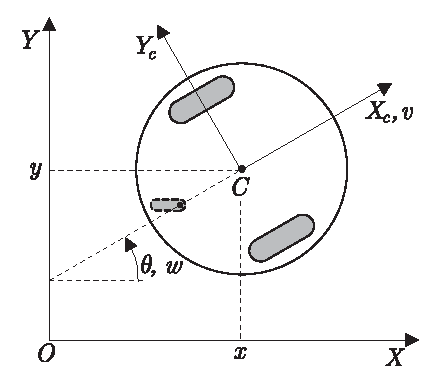
\includegraphics[width=0.67\linewidth]{Figuras/robot.eps}
	\caption{Coordinate system of the WMR.}
	\label{fig:robot}
\end{figure}

For the sake of simplicity, we assume in this work that the states of the plant are always available for measurement and that there are no plant/model mismatch.

As we will se in the next sections, in MPC a prediction model is used and the control law is computed in discrete-time. Thus, a discrete-time representation of this model becomes necessary. Considering a simpling period $T$ and applying the Euler's approximation, to Eq.~\req{eqn:model}, we obtain the following discrete-time model for the robot motion:
\begin{equation}
\label{eqn:discretemodel}
	\left\{
		\begin{aligned}
			x(k+1)	    &= x(k) + v(k)\cos\theta(k)T \\
			y(k+1)	    &= y(k) + v(k)\sin\theta(k)T \\
			\theta(k+1) &= \theta(k) + w(k)T \\
		\end{aligned}
	\right.
\end{equation}
or, in a compact representation,
\begin{equation}\label{eqn:discretemodelshort}
	{\bf x}(k+1) = f_d({\bf x}(k),{\bf u}(k))
\end{equation}

The problem of trajectory tracking of a mobile robot can be stated as to find a control law such that
\begin{equation*}
	{\bf x}(t)-{\bf x}_r=0
\end{equation*}
where ${\bf x}_r$ is a previously known reference trajectory. It is usual to associate to this reference trajectory a {\em virtual} reference model, which has the same model of the robot to be controlled. Thus, we have:
\begin{equation}\label{eqn:refmodel}
	\dot{\bf x}_r = f({\bf x}_r,{\bf u}_r),
\end{equation}
or, in discrete-time, ${\bf x}_r(k+1) = f_d({\bf x}_r(k),{\bf u}_r(k))$.


%%%%%%%%%%%%%%%%%%%%%%%%%%%%%%%%%%%%%%%%%%%%%%%%%%%%
\section{The Nonlinear MPC Approach}\label{sec:nmpc}
In this section, the trajectory tracking problem is solved with a NMPC strategy, and some simulations results will be shown.

As pointed out in Section~\ref{sec:intro}, the essence of a MPC scheme is to optimize predictions of process behavior over a sequence of future control inputs. Such a prediction is accomplished by using a process model over a finite time
interval, called the {\em prediction horizon}. At each sampling time, the model predictive controller generates an optimal control sequence by solving an optimization problem. The first element of this sequence is applied to the
plant. The problem is solved again at the next sampling time using the updated process measurements and a shifted horizon.

Considering a robot described by Eq.~\req{eqn:discretemodelshort}, the following prediction model can be formulated:
\begin{equation*}
	{\bf x}(k+j+1|k)=f_d({\bf x}(k+j|k),{\bf u}(k+j|k)),
\end{equation*}
where $j\in[0,N-1]$ and the notation $a(m|n)$ indicates the value of $a$ at the instant $m$ predicted at instant $n$. Furthermore, let us consider the existence of bounds in the amplitude of the control variables:
\begin{equation}\label{eqn:restu}
	{\bf u}_{min} \leq {\bf u}(k+j|k) \leq {\bf u}_{max},
\end{equation}
where, once more, $j\in[0,N-1]$. By defining error vectors $\tilde{\bf x}={\bf x}-{\bf x}_r$ and $\tilde{\bf u}={\bf u}-{\bf u}_r$, we can formulate the following objective function to be minimized:
\begin{multline}\label{eqn:cost}
	\Phi(k) = \sum_{j=1}^{N}\tilde{\bf x}^T(k+j|k){\bf Q}\tilde{\bf x}(k+j|k) + \\ + \tilde{\bf u}^T(k+j-1|k)\tilde{\bf R}{\bf u}(k+j-1|k),
\end{multline}
where $N$ is the prediction horizon and ${\bf Q}$, ${\bf R}$ are weighting matrices, with ${\bf Q}\geq 0$ and ${\bf R}>0$.

Hence, the nonlinear optimization problem can therefore be stated as to find $\tilde{\bf u}^\star$ such that:
\begin{equation}\label{eqn:optim}
	{\bf x}^\star,{\bf u}^\star = \arg\min_{{\bf x},{\bf u}}\left\{\Phi(k)\right\}
\end{equation}
s. a.
\begin{align}
	{\bf x}(k|k)     &= {\bf x}_0, \label{eqn:restci} \\
	{\bf x}(k+j+1|k) &= f_d({\bf x}(k+j|k),{\bf u}(k+j|k)), \label{eqn:restmodel} \\
	{\bf Du}(k+j|k)  &\leq {\bf d}, \label{eqn:restgu}
\end{align}
where ${\bf x}_0$ in Eq.~\req{eqn:restci} is the measured initial condition. Notice that the decision variables are both state and control variables. Eq.~\req{eqn:restgu} is a general way to write linear constraints in the control inputs, such as Eq.~\req{eqn:restu}.

Then, the optimization problem~\req{eqn:optim}--\req{eqn:restgu} is solved at each sampling time $k$, yielding a sequence of optimal state $\{{\bf x}^\star(k+1|k),\ldots,{\bf x}^\star(k+N|k)\}$, optimal control $\{{\bf u}^\star(k|k),\ldots,{\bf u}^\star(k+N-1|k)\}$ and the optimal cost $\Phi^\star(k)$. The MPC control law is implicitly given by the first control action of the sequence of optimal control, ${\bf u}^\star(k|k)$.

\begin{ex}\label{ex1}
Considering a robot described by Eq.~\ref{eqn:model}, the optimization problem ~\req{eqn:optim}--\req{eqn:restgu} is solved to the problem of trajectory tracking. Constraints in the amplitude of the control variables are $v_{max}=0.47~m/s$, $v_{min}=-0.47~m/s$, $w_{max}=3.77~rad/s$ and $w_{min}=-3.77~rad/s$. Hence, we have
\begin{equation*}
	{\bf D} = \begin{bmatrix} {\bf I} \\ -{\bf I} \end{bmatrix}, \qquad 
	{\bf d} = \begin{bmatrix} 0.47~m/s \\ 3.77~rad/s \\ 0.47~m/s \\ 3.77~rad/s \end{bmatrix}
\end{equation*}
in Eq.~\req{eqn:restgu}. Using a reference trajectory in "U" form and with the tunning parameters: $N=5$, ${\bf Q}={\rm diag}(1;1;0,5)$, ${\bf R}={\rm diag}(0,1;0,1)$ and with a initial condition of ${\bf x}_0=[-1~~-1~~0]^T$, we have the simulation results\footnote{The {\sc Matlab} routine {\tt fmincon} has been used to solve the optimization problem.} shown in Fig's~\ref{fig:traj_01} and \ref{fig:control_01}.
\begin{figure}[H]
	\centering
   	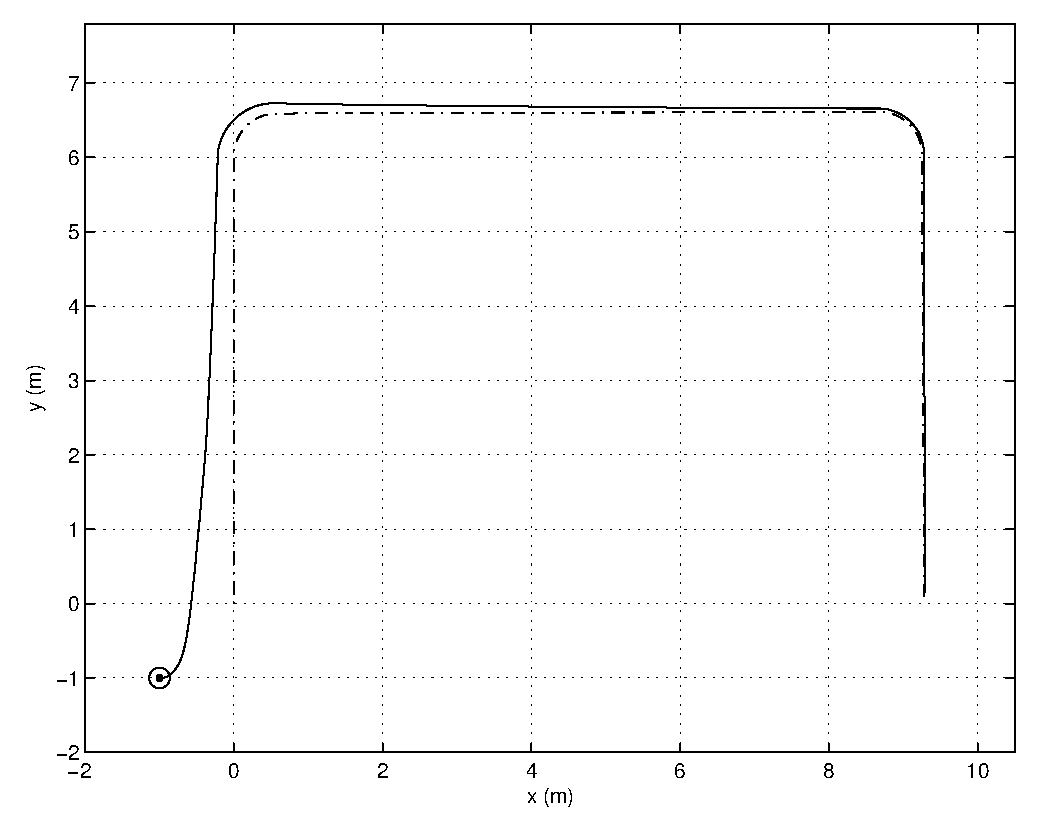
\includegraphics[width=.9\linewidth]{Figuras/traj_01.eps}
    	\caption{Trajectory in the $XY$ plane.}
    	\label{fig:traj_01}
\end{figure}
\begin{figure}[htbp]
	\centering
    	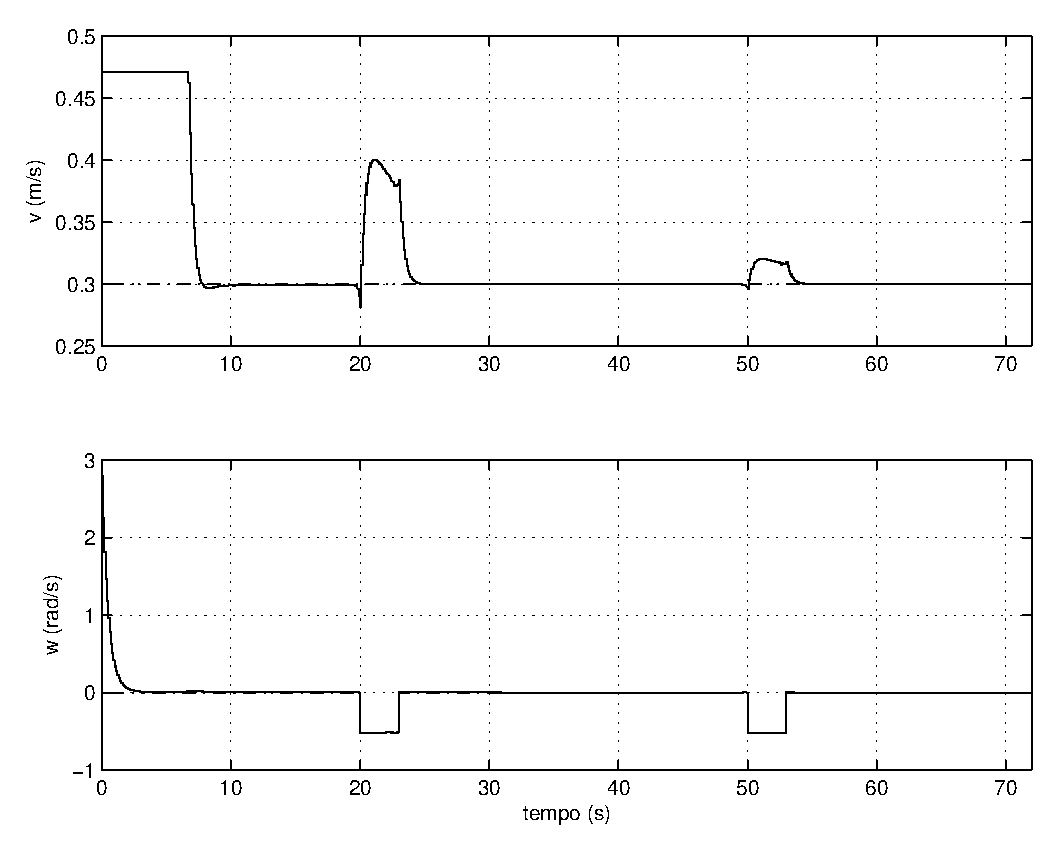
\includegraphics[width=.9\linewidth]{Figuras/control_01.eps}
    	\caption{Controls inputs.}
	\label{fig:control_01}
\end{figure}

It can be noted in Fig.~\ref{fig:traj_01} that the problem is successfully solved, but with low convergence rate. Fig.~\ref{fig:control_01} shows the control inputs bounded by the imposed constraints. The dash-dotted lines stands for the reference trajectories.
\fimex
\end{ex}

The convergence rate can be improved by introducing some modifications in the cost function to be minimized. In~\cite{essen01} the idea of exponentially increasing wheighting factors in the state variable is introduced. Furthermore, a terminal state cost is added. Thus, the following cost function can be formulated:
\begin{multline}\label{eqn:essencost}
	\Phi(k) = \sum_{j=1}^{N-1}\tilde{\bf x}^T(k+j|k){\bf Q}(j)\tilde{\bf x}(k+j|k) + \\ + \sum_{j=0}^{N-1}\tilde{\bf u}^T(k+j|k){\bf R}\tilde{\bf u}(k+j|k) + \Omega(\tilde{\bf x}(k+N|k)),
\end{multline}
where ${\bf Q}(j) = 2^{j-1}{\bf Q}$ and $\Omega(\tilde{\bf x}(k+N|k)) = \tilde{\bf x}^T(k+N|k){\bf P}\tilde{\bf x}(k+N|k)$ is the terminal state cost.

\begin{ex}\label{ex2}
Thus, by using the same conditions of Example~\ref{ex1} with ${\bf P}=30{\bf Q}(N)$, we have the results shown in Fig's~\ref{fig:traj_02} and \ref{fig:control_02}.
\begin{figure}[htbp]
	\centering
   	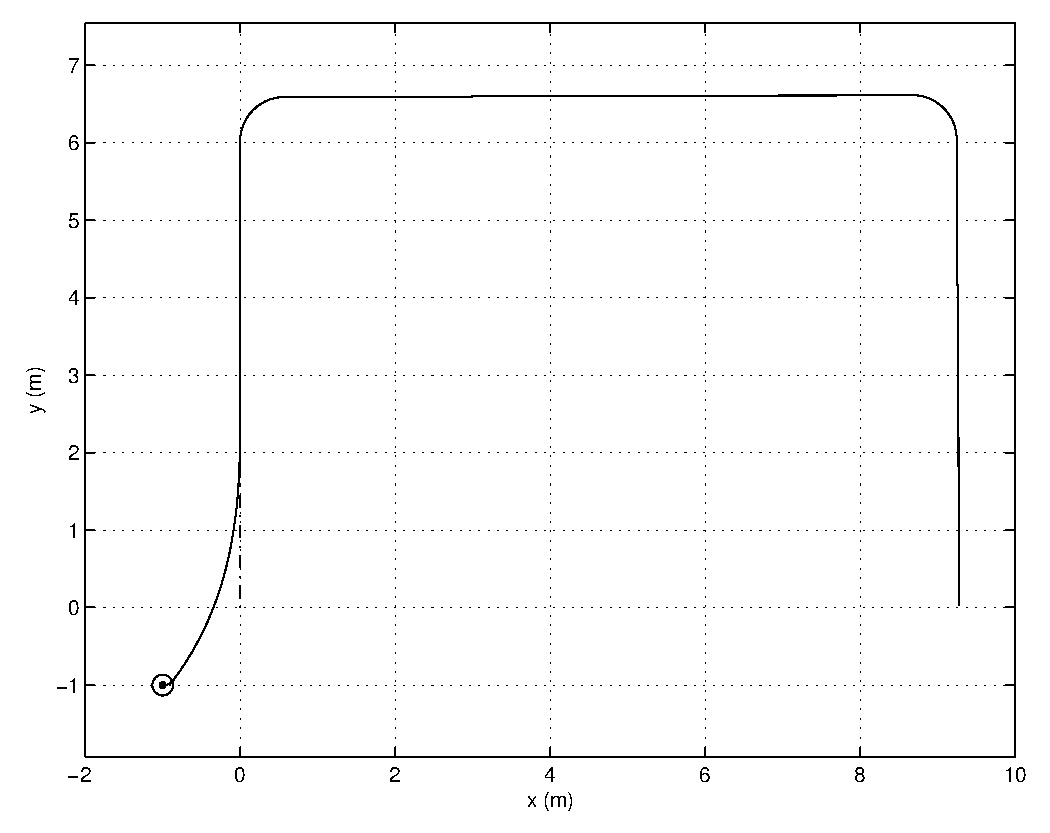
\includegraphics[width=.9\linewidth]{Figuras/traj_02.eps}
    	\caption{Trajectory in the $XY$ plane.}
    	\label{fig:traj_02}
\end{figure}
\begin{figure}[htbp]
	\centering
    	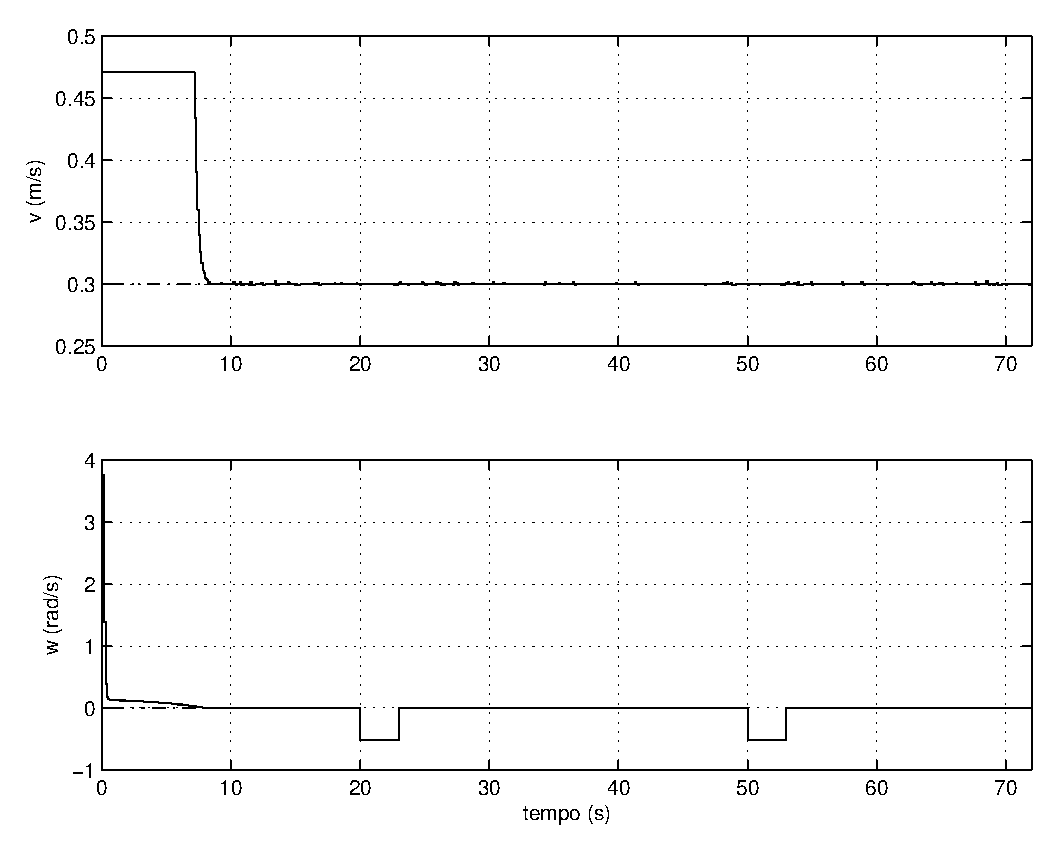
\includegraphics[width=.9\linewidth]{Figuras/control_02.eps}
    	\caption{Controls inputs.}
	\label{fig:control_02}
\end{figure}

Thus, comparing Fig.~\ref{fig:traj_01} and \ref{fig:traj_02}, it can be clearly seen that the robot presents a higher convergence rate, and Fig.~\ref{fig:control_02} shows that the control signals respect the constraints imposed.
\fimex
\end{ex}


%%%%%%%%%%%%%%%%%%%%%%%%%%%%%%%%%%%%%%%%%%%%%%%%%
\section{The Linear MPC Approach}\label{sec:lmpc}
In this section we will introduce a linear MPC (LMPC) scheme applied to the problem of trajectory tracking.

Although NMPC has been well developed~\cite{chen98,allgower99}, the computational effort necessary is much higher than the linear version. In NMPC there is a nonlinear programming problem to be solved on-line, which is nonconvex, has a larger number of decision variables and a global minimum is in general impossible to find~\cite{henson98}. In this section, we propose a strategy in order to reduce the computational cost. The fundamental idea consists in using a successive linearization approach, yielding a linear, time-varying description of the system beeing solved through linear MPC. Then, considering the control inputs as the decision variables, it is possible to transform the optimization problem in a QP problem. Since they are convex, QP problems can be easily solved by numerically robust algorithms which lead to global optimal solutions.

A linear model of the system's dynamics can be obtained by computing an error model with respect to a reference car. To do so, consider the reference car described by~\req{eqn:refmodel}.

By expanding the right side of \req{eqn:modelshort} in Taylor series around the point $({\bf x}_r,{\bf u}_r)$ and discarding the high order terms it follows that
\begin{multline*}\label{eqn:taylor2}
\dot{\bf x} = f({\bf x}_r,{\bf u}_r) + \left.\frac{\partial f({\bf x},{\bf u})}{\partial{\bf x}}\right|_{\begin{smallmatrix}{\bf x}={\bf x}_r \\
{\bf u}={\bf u}_r \end{smallmatrix}}({\bf x}-{\bf x}_r) + \\
+ \left.\frac{\partial f({\bf x},{\bf u})}{\partial{\bf u}}\right|_{\begin{smallmatrix}{\bf x}={\bf x}_r \\
{\bf u}={\bf u}_r \end{smallmatrix}}({\bf u}-{\bf u}_r),
\end{multline*}
or
\begin{equation}\label{eqn:taylor}
	\dot{\bf x} = f({\bf x}_r,{\bf u}_r) + f_{{\bf x},r}({\bf x}-{\bf x}_r) + f_{{\bf u},r}({\bf u}-{\bf u}_r),
\end{equation}
where $f_{{\bf x},r}$ and $f_{{\bf u},r}$ are the jacobians of $f$ with respect to ${\bf x}$ and ${\bf u}$, respectively, evaluated around the reference point $({\bf x}_r,{\bf u}_r)$.
Then, the subtraction of~\req{eqn:refmodel} from~\req{eqn:taylor} results in:
\begin{equation*}\label{eqn:conterror}
	{\dot{\tilde{\bf x}}} = f_{{\bf x},r}\tilde{\bf x}+f_{{\bf u},r}\tilde{\bf u},
\end{equation*}
where, $\tilde{\bf x}={\bf x}-{\bf x}_r$ represents the error with respect to the reference car and $\tilde{\bf u}={\bf u}-{\bf u}_r$ is its associated perturbation control input.

The approximation of $\dot{\bf x}$ by using forward differences gives the following discrete-time system model:

\begin{equation}
\label{eqn:error}
	\tilde{\bf x}(k+1) = {\bf A}(k)\tilde{\bf x}(k)+{\bf B}(k)\tilde{\bf u}(k),
\end{equation}
with
\begin{align*}
	{\bf A}(k) &= \begin{bmatrix}
		1 & 0 & -v_r(k)\sin\theta_r(k)T \\
		0 & 1 &  v_r(k)\cos\theta_r(k)T \\
		0 & 0 & 1
	\end{bmatrix} \\
	{\bf B}(k) &= \begin{bmatrix}
		\cos\theta_r(k)T & 0 \\
		\sin\theta_r(k)T & 0 \\
		0 			  & T
	\end{bmatrix}
\end{align*}
where $T$ is the sampling period and $k$ is the sampling time.

In~\cite{bloch89} it is shown that the nonlinear, nonholonomic system~\req{eqn:model} is fully controllable, i.e., it can be steered from any initial state to any final state in finite time by using finite inputs. On the other hand, it is easy to see that when the robot is not moving, the linearization about a stationary operating point is not controllable. However, this linearization becomes controllable as long as the control input ${\bf u}$ is not zero~\cite{samson91}. This implies the tracking of a reference trajectory being possible with linear MPC~\cite{essen01}.

Now it is necessary to recast the optimization problem in an usual quadratic programming form. Hence, we introduce the following vectors:
\begin{equation*}
	\bar{\bf x}(k+1) = \begin{bmatrix}
		\tilde{\bf x}(k+1|k) \\ \tilde{\bf x}(k+2|k) \\ \vdots \\ \tilde{\bf x}(k+N|k) 
	\end{bmatrix},~
	\bar{\bf u}(k) = \begin{bmatrix}
		\tilde{\bf u}(k|k)  \\ \tilde{\bf u}(k+1|k) \\ \vdots \\ \tilde{\bf u}(k+N-1|k)
	\end{bmatrix}
\end{equation*}

Thus, with $\overline{\bf Q}={\rm diag}({\bf Q};\ldots;{\bf Q})$ and $\overline{\bf R}={\rm diag}({\bf R};\ldots;{\bf R})$, the cost function~\req{eqn:cost} can be rewritten as~\cite{kuhne05}:
\begin{equation}\label{eqn:cost2}
	\Phi(k) = \bar{\bf x}^T(k+1)\bar{\bf Q}\bar{\bf x}(k+1) + \bar{\bf u}^T(k)\bar{\bf R}\bar{\bf u}(k),
\end{equation}

Therefore, it is possible from~\req{eqn:error} to write $\bar{\bf x}(k+1)$ as:
\begin{equation}\label{eqn:exbar}
	\bar{\bf x}(k+1) = \bar{\bf A}(k)\tilde{\bf x}(k|k)+\bar{\bf B}(k)\bar{\bf u}(k),
\end{equation}
%with
%\begin{equation*}
%	\bar{\bf A}(k) = \begin{bmatrix}
%		{\bf A}(k|k) \\ {\bf A}(k|k){\bf A}(k+1|k) \\ \vdots \\ \alpha(k,0,2) \\ \alpha(k,0,1)
%	\end{bmatrix}
%\end{equation*}
%and
%{\tiny
%\begin{multline*}
%		\bar{\bf B}(k) = \\ \begin{bmatrix}
%			{\bf B}(k|k)		       & {\bf 0} 			    	  & \cdots & {\bf 0}         \\
%			{\bf A}(k+1|k){\bf B}(k|k) & {\bf B}(k+1|k)      	       & \cdots & {\bf 0}         \\
%			\vdots			       & \vdots			  	  & \ddots & \vdots          \\
%			\alpha(k,1,2){\bf B}(k|k)  & \alpha(k,2,2){\bf B}(k+1|k) & \cdots & {\bf 0}	    \\
%			\alpha(k,1,1){\bf B}(k|k)  & \alpha(k,2,1){\bf B}(k+1|k) & \cdots & {\bf B}(k+N-1|k)
%		\end{bmatrix}
%\end{multline*}
%}
%where $\alpha(k,j,l)$ is defined as:
%\begin{equation*}
%	\alpha(k,j,l) = \prod_{i=j}^{N-l}{\bf A}(k+i|k)
%\end{equation*}

From~\req{eqn:cost2} and~\req{eqn:exbar}, after some algebraic manipulations (refers to~\cite{kuhne05} for more details), we can rewrite the objective function~\req{eqn:cost} in a standard quadratic form:
\begin{equation}\label{eqn:cost3}
	\overline\Phi(k) = \frac{1}{2}\bar{\bf u}^T(k){\bf H}(k)\bar{\bf u}(k) + {\bf f}^T(k)\bar{\bf u}(k) + {\bf d}(k)
\end{equation}
with
\begin{align*}
	{\bf H}(k) &= 2\left(\bar{\bf B}(k)^T(k)\bar{\bf Q}\bar{\bf B}(k)+\bar{\bf R}\right) \\
	{\bf f}(k) &= 2\bar{\bf B}^T(k)\bar{\bf Q}\bar{\bf A}(k)\tilde{\bf x}(k|k) \\
	{\bf d}(k) &= \tilde{\bf x}^T(k|k)\bar{\bf A}^T(k)\bar{\bf Q}\bar{\bf A}(k)\tilde{\bf x}(k|k)
\end{align*}

The matrix ${\bf H}$ is a {\em Hessian} matrix, and must be positive definite. It describes the quadratic part of the objective function, and the vector ${\bf f}$ describes the linear part. $\bf d$ is independent of $\tilde{\bf u}$ and has no influence in the determination of $\bf u^\star$.

It this case, the optimization problem to be solved at each sampling time is stated as follows:
\begin{equation}\label{eqn:optim2}
	\tilde{\bf u}^\star = \arg\min_{\tilde{\bf u}}\left\{\overline\Phi(k)\right\}
\end{equation}
s. a.
\begin{equation}\label{eqn:restu2}
	{\bf D\tilde u}(k+j|k) \leq {\bf d}, ~~j~\in[0,N-1]
\end{equation}

Notice that now only the control variables are used as decision variables. Furthermore, constraints for the initial condition and model dynamics are not necessary anymore, since now these informations are implicit in the cost function~\req{eqn:cost3}, and any constraint must be written with respect to the decision variables (Eq.~\req{eqn:restu2}). In this case, the amplitude constraints in the control variables ${\bf u}_{min}\leq{\bf u}(k)\leq{\bf u}_{max}$ can be rewritten as:
\begin{equation}\label{eqn:resttilu}
	{\bf u}_{min} - {\bf u}_r(k) \leq \tilde{\bf u}(k) \leq {\bf u}_{max} - {\bf u}_r(k),
\end{equation}

Since the state prediction is a function of the optimal sequence to be computed, it is easy to show that state constraints can also be described generically by Eq.~\req{eqn:restu2}. Furthermore, constraints on the control rate and states can be formulated in a similar way.

\begin{ex}\label{ex3}
Using the procedure described above, The cost function~\req{eqn:essencost}~\cite{essen01} is recasted as Eq.~\req{eqn:cost3}. Considering the same data as in Example~\ref{ex2}, the optimization problem~\req{eqn:optim2}--\req{eqn:restu2} is solved at each sampling time. Since now the constraints are written with relation to $\tilde{\bf u}$, according to Eq.~\req{eqn:resttilu} we have that:
\begin{equation*}
	{\bf D} = \begin{bmatrix} {\bf I} \\ -{\bf I} \end{bmatrix}, \qquad 
	{\bf d} = \begin{bmatrix} 0.47~m/s-v_r(k) \\ 3.77~rad/s-w_r(k) \\ 0.47~m/s+v_r(k) \\ 3.77~rad/s+w_r(k) \end{bmatrix}
\end{equation*}

Then, we have in Fig's~\ref{fig:traj_03}--\ref{fig:control_03} the simulation results\footnote{The optimization problem was solved with the {\sc Matlab} routine {\tt quadprog}.}, where the dash-dotted lines stand for the reference trajectories and the dotted line stand for the trajectories of the nonlinear case (Fig's~\ref{fig:traj_02} and \ref{fig:control_02}).
\begin{figure}[htbp]
	\centering
   	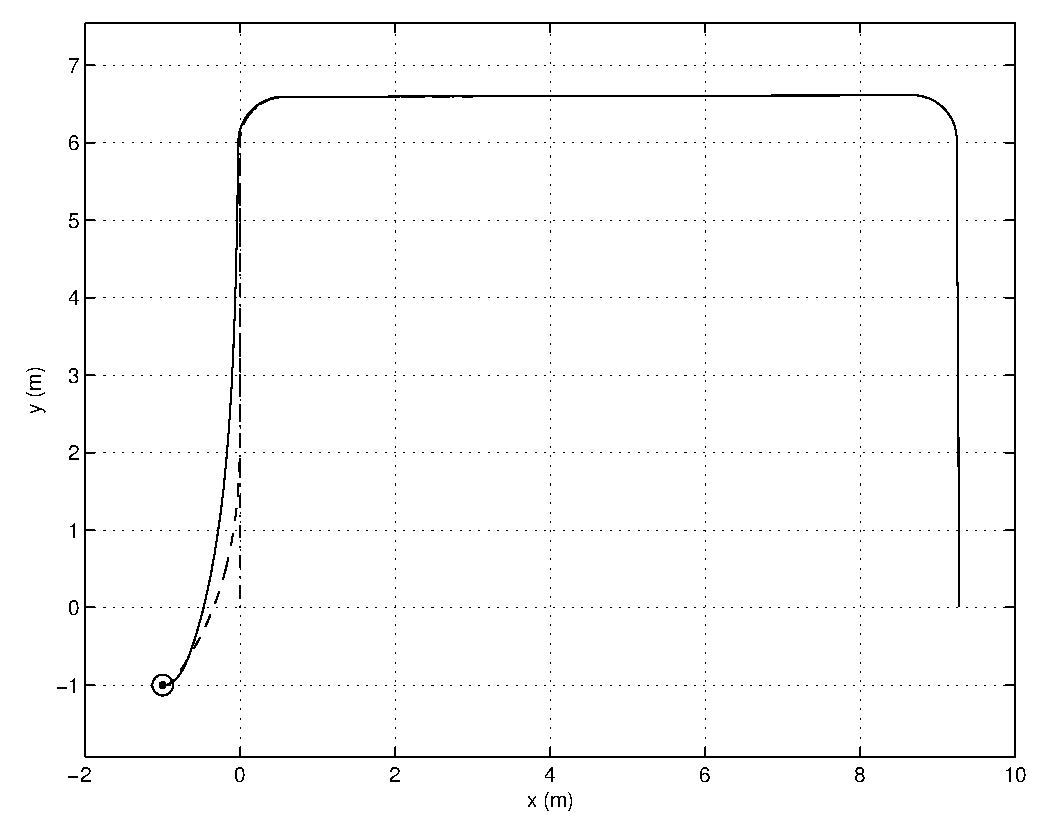
\includegraphics[width=.9\linewidth]{Figuras/traj_03.eps}
    	\caption{Trajectory in the $XY$ plane.}
    	\label{fig:traj_03}
\end{figure}
\begin{figure}[htbp]
	\centering
    	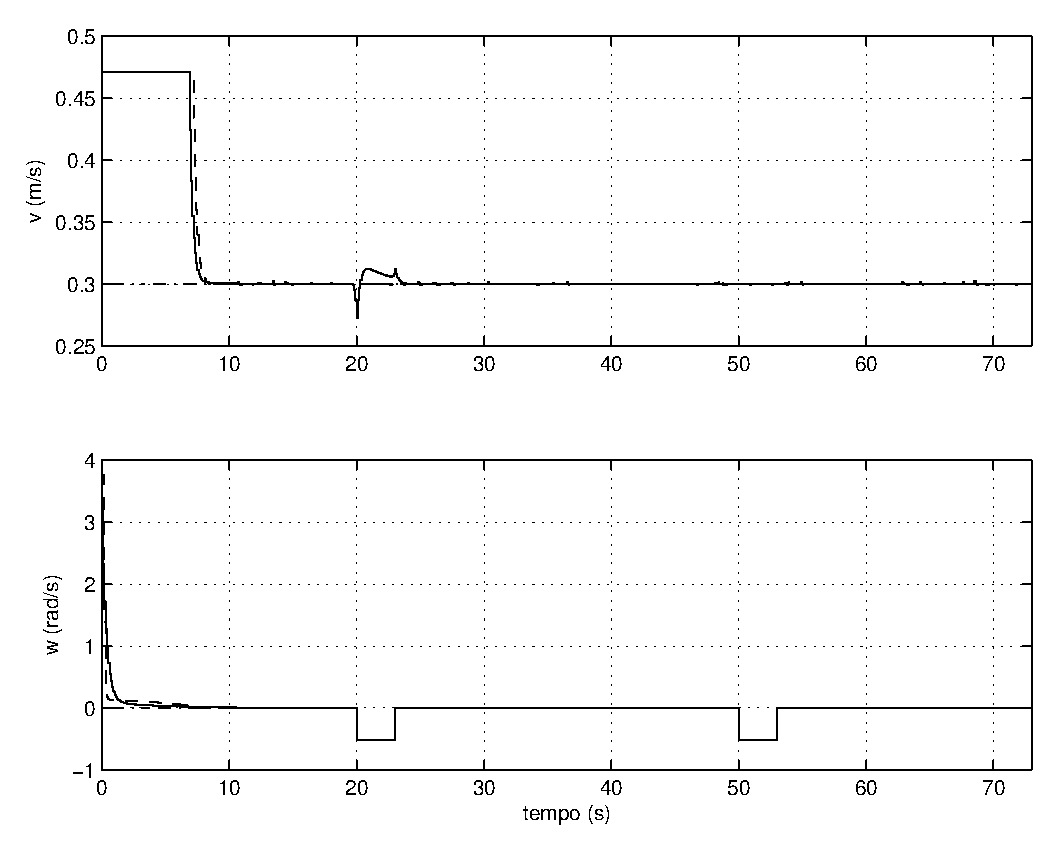
\includegraphics[width=.9\linewidth]{Figuras/control_03.eps}
    	\caption{Controls inputs.}
	\label{fig:control_03}
\end{figure}

It is esay to notice that there are not significative difference between the nonlinear (Fig's~\ref{fig:traj_02} and \ref{fig:control_02}) and linear cases (Fig's~\ref{fig:traj_03} and \ref{fig:control_03}). Once more, the control signals are such that respect the constraints imposed. 
\fimex
\end{ex}

%%%%%%%%%%%%%%%%%%%%%%%%%%%%%%%%%%
\section{The Computational Effort}
The use of MPC for real-time control of systems with fast dynamics such as a WMR has been hindered for some time due to its numerical intensive nature~\cite{cannon00}. However, with the development of increasingly faster processors the use of MPC in demanding applications becomes possible. 

Then, some analyses are now developed with the purpose of speculating the viability of the application of the proposed techniques in a real implementation. For such task, the number of floating-point operations per second (flops) needed to solve the optimization problems will be used as an evaluation criterion.

For example, let us consider a computer with an Athlon XP 2600+ processor, which gives a peak performance between 576 and 1100 Mflops using double precision computations accordingly to~\cite{aburto92}, a de-facto standard for floating point performance measurement.

The sampling period used in all examples presented here is $T=100~ms$. The data in Table~\ref{tab:cost} refers to the mean values along the trajectory, and it provides enough evidence that a standard of-the-shelf computer is able to run a MPC-based controller for a WMR.

It is important to note the difference between the nonlinear and linear cases. For a horizon higher than 10, the NMCP would not be applicable, while the LMPC presents admissible computational effort for a horizon of 20 or even higher. On the other hand, comparing the performance showed in Fig.~\ref{fig:traj_03} and Table~\ref{tab:cost}, we can say that the linear approach developed here is a good alternative when lower computational effort is necessary while it does not presents a significative lost in performance.


\begin{table}[H]
	\renewcommand{\arraystretch}{1.2}
	\label{tab:cost}
	\caption{The computational effort.}
	\centering
 	\begin{tabular}{c|cc}
  		\hline
  				& \multicolumn{2}{c}{Mflops} \\
          Horizon 	& NMPC & LMPC \\
  		\hline\hline
  		5	& 11.1 & 0.17 \\
  		10	& 502 & 0.95 \\
  		15	& 5364 & 3.5 \\
  		20	& --- & 9.1  \\
  		\hline
 	\end{tabular}
\end{table}


%%%%%%%%%%%%%%%%%%%%%%%%%%%%%%%%%%%%%%%%%%%
\section{Conclusion}\label{sec:conclusions}

This paper presented an application of MPC to the problem of trajectory tracking of a differential-drive, nonholonomic WMR. The solution of the optimization problem through nonlinear and linear method was shown. The obtained control signals were such that the constraints imposed on the control variables were respected and the convergence rates were improved by some modifications in the cost function. 

In the sequel, a study about the computational effort needed to solve the optimization problems was carried out, where the number of flops was used as evaluation criterion.

With the linear approach, it has been possible to reduce the computational effort, since the MPC has been recasted as a QP formulation. In comparison with the nonlinear approach, it has been noticed that the linear strategy mantains good performance, with lower computational effort. It is important to point out that the LMPC has the disadvantage that the linearized model is only valid for points near the reference trajectory. However, this problem can be easily solved with the {\em pure-pursuit} strategy~\cite{rico99}.

As shown above, the choice of MPC for the application given here is well justified by some advantages: the straightforward way in which state/input constraints can be handled; the existence of a performance criterion to be minimized; the tunning parameters are easy and intuitive to deal with.

%%%%%%%%%%%%%%%%%%%%%%%%%%
\section*{Acknowledgments}
The authors gratefully acknowledge the financial support from CAPES.


\bibliography{sbai05}

\end{document}
